% The new draft's supplied vector curves and axes are retained exactly.
% Only panel titles and legend wording are re-typeset for consistency.
\begin{tikzpicture}[x=1bp,y=-1bp]
\useasboundingbox (0,0) rectangle (248.4,106.56);
\node[anchor=north west,inner sep=0pt] at (0,0)
  {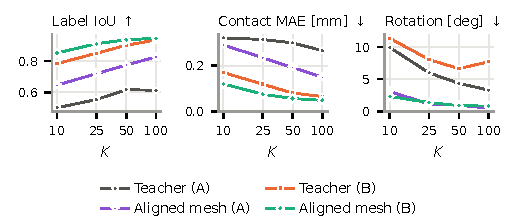
\includegraphics[width=248.4bp]{figures/src/label_quality_curves.pdf}};
\node[anchor=north,inner sep=0pt,font=\fontsize{6.7bp}{8bp}\selectfont] at (50.6,4.8) {Label IoU $\uparrow$};
\node[anchor=north,inner sep=0pt,font=\fontsize{6.7bp}{8bp}\selectfont] at (131.3,4.8) {Contact MAE (mm) $\downarrow$};
\node[anchor=north,inner sep=0pt,font=\fontsize{6.7bp}{8bp}\selectfont] at (211.7,4.8) {Rotation (deg) $\downarrow$};
\node[anchor=base west,inner sep=0pt,font=\fontsize{6.7bp}{8bp}\selectfont] at (43.75,92.7) {Teacher (A)};
\node[anchor=base west,inner sep=0pt,font=\fontsize{6.7bp}{8bp}\selectfont] at (43.75,102.45) {Aligned mesh (A)};
\node[anchor=base west,inner sep=0pt,font=\fontsize{6.7bp}{8bp}\selectfont] at (143.7,92.7) {Teacher (B)};
\node[anchor=base west,inner sep=0pt,font=\fontsize{6.7bp}{8bp}\selectfont] at (143.7,102.45) {Aligned mesh (B)};
\node[anchor=base,inner sep=0pt,font=\fontsize{8bp}{10bp}\selectfont] at (50.69,75.35) {$K$};
\node[anchor=base,inner sep=0pt,font=\fontsize{8bp}{10bp}\selectfont] at (130.77,75.35) {$K$};
\node[anchor=base,inner sep=0pt,font=\fontsize{8bp}{10bp}\selectfont] at (210.85,75.35) {$K$};
\end{tikzpicture}
